
% !TeX spellcheck = pt_BR
% !TEX encoding = UTF-8 Unicode

% Ver copyright.tex para direitos autorais e licença.

\clearpage
\section{Coeficiente de Correlação}

A covariância é uma quantidade útil que descreve como duas variáveis aleatórias variam juntas. No entanto, ela tem uma desvantagem: não é invariante à escala. Para explicar o que isso significa, suponha que $X$ e $Y$ sejam duas variáveis aleatórias, ambas medindo comprimentos em metros. Vamos assumir que $U$ e $V$ fornecem as mesmas medidas que $X$ e $Y$, respectivamente, mas em centímetros, ou seja, $U = 100X$ e $V = 100Y$. Então,
\[\Cov(U, V) = \Cov(100X, 100Y) = 100 \cdot 100 \cdot \Cov(X, Y) = 10^4 \cdot \Cov(U, V).\]
Isso significa que alterar a escala também altera a covariância. Para obter uma quantidade invariante à escala, fazemos a seguinte definição.

\begin{definition*}
[Coeficiente de Correlação]
Sejam $X$ e $Y$ variáveis aleatórias discretas quadrado-integráveis com variância positiva. O \emph{coeficiente de correlação} entre $X$ e $Y$ é definido como
\[
\rho(X, Y) = \frac{\Cov(X, Y)}{\sigma(X) \cdot \sigma(Y)}
.
\]
\end{definition*}

Conforme prometido, o coeficiente de correlação não muda quando escalamos ou deslocamos as variáveis aleatórias.

\begin{proposition*}
Sejam $X$ e $Y$ variáveis aleatórias quadrado-integráveis com variância positiva. Para qualquer $a, b, c, d \in \R$ com $a, c > 0$, temos
\[
\rho(aX + b, cY + d) = \rho(X, Y)
.
\]
\end{proposition*}
\begin{proof}
Primeiro, observamos que a covariância entre uma constante e qualquer outra variável aleatória é igual a zero. De fato,
\[
\Cov(b, Y) = \E[bY] - \E[b] \cdot \E[Y] = b \cdot \E[Y] - b \cdot \E[Y] = 0
.
\]
Portanto,
%\begin{align*}
%\Cov(aX+b,cY+d) = ac\cdot\Cov(X,Y)
% +c\cdot\Cov(b,Y)+a\cdot\Cov(X,d) + \Cov(b,d).
%\end{align*}
%Então, obtemos a partir disso que
\[\Cov(aX + b, cY + d) = ac \cdot \Cov(X, Y).\]
Substituindo isso na fórmula do coeficiente de correlação,
\begin{align*}
\rho(aX + b, cY + d)
&=
\frac{\Cov(aX + b, cY + d)}{{\sigma(aX + b) \cdot \sigma(cY + d)}}
\\
&=
\frac{ac \cdot \Cov(X, Y)}{{a \cdot \sigma(X) \cdot c \cdot \sigma(Y)}}
\\
&=
\frac{\Cov(X, Y)}{{\sigma(X) \cdot \sigma(Y)}}
= \rho(X, Y)
.
\qedhere
\end{align*}
\end{proof}

Além disso, como $\sigma(-Y) = \sigma(Y)$ e $\Cov(X, Y) = \Cov(Y, X)$, o coeficiente de correlação também satisfaz.
\[
\rho(X, Y) = \rho(Y, X)
\text{ e }
\rho(X, -Y) = -\rho(X, Y)
.
\]

A próxima proposição descreve ainda mais em que sentido o coeficiente de correlação $\rho(X, Y)$ é um índice adimensional que quantifica o quão bem $X$ e $Y$ estão alinhados, veja a Figura~\ref{fig:Correlation_examples2} para uma descrição visual.

\begin{figure}[b!]
\includegraphics[width=\textwidth]{Pictures/Correlation_examples2}
\caption{Ilustração de $ \rho(X,Y) $ assumindo que o par $ (X, Y) $ tem a mesma probabilidade de estar em cada ponto na nuvem representada. \hfill (retirado da Wikipedia)}
\label{fig:Correlation_examples2}
\end{figure}

\begin{proposition*}
Sejam $X$ e $Y$ variáveis aleatórias quadrado-integráveis com variância positiva.
Então
\[
-1 \le \rho(X, Y) \le 1
.
\]
Nos casos extremos, $\rho(X, X) = 1$ e $\rho(X, -X) = -1$.
\end{proposition*}
\begin{proof}
Observe que
\[
\left(\frac{X-\E[X]}{\sigma(X)} - \frac{Y-\E[Y]}{\sigma(Y)}\right)^2\geq 0
\]
Tomando a expectativa e expandindo, obtemos
\[
\frac{\E[(X-\E[X])^2]}{\sigma^2(X)} + \frac{\E[(Y-\E[Y])^2]}{\sigma^2(Y)} - 2\frac{\E[(X-\E[X])(Y-\E[Y])]}{\sigma(X)\sigma(Y)}
\geq
0
,
\]
o que significa
\[
2 \rho(X,Y) \leq 2,
\]
logo
$ \rho(X,Y) \leq 1 $.
O mesmo argumento com $ -Y $ no lugar de $ Y $ nos dá $ \rho(X,Y) = -\rho(X,-Y) \leq 1 $, portanto
$ \rho(X,Y) \geq -1 $.
Finalmente,
\[
\rho(X,X) = \frac{\Cov(X,Y)}{\sigma(X)\cdot\sigma(X)} = 1
\]
e $ \rho(X,-X) = - \rho(X,X) = -1 $.
\end{proof}

\clearpage
\section{Teorema do Limite Central}

\begin{theorem}
[Teorema do Limite Central]
Sejam $ X_1,X_2,X_3,\dots $ variáveis aleatórias independentes entre si, quadrado-integráveis, com a mesma distribuição. Denote sua média por $ \mu $ e variância por $ \sigma^2 > 0 $.
Então, para todo $ a<b $
\[
\Pb\Big( a \leq \frac{X_1+\dots+X_n - n\cdot \mu}{\sigma \cdot \sqrt{n}} \leq b \Big)
\approx
\int_a^b
\tfrac{1}{\sqrt{2 \pi}}
e^{-x^2/2} \, \dd x
.
\]
\end{theorem}
A aproximação ``$ {\approx} $'' significa que a probabilidade se aproxima o quanto desejarmos da integral (como mostrado na Figura~\ref{fig:normalarea}) se escolhermos $ n $ suficientemente grande.

Esse fenômeno notável está no cerne da estatística e da maioria das ciências naturais.
Ele afirma que, \emph{independentemente da distribuição de $ X $}, se adicionarmos um número suficiente de amostras de $ X $, só veremos sua média $ \mu $ e variância $ \sigma^2 $.

\begin{figure}[b!]
\centering
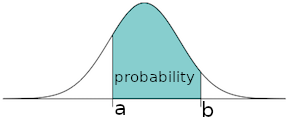
\includegraphics[width=.5\textwidth]{Pictures/normalarea}
\caption{Gráfico de $ y = \frac{1}{\sqrt{2\pi}}e^{-x^2/2} $ e a probabilidade de que $ Z \in [a,b] $ representada pela área esverdeada entre os pontos $ a $ e $ b $.}
\label{fig:normalarea}
\end{figure}

Não demonstraremos o Teorema do Limite Central neste módulo, pois são necessárias ferramentas mais avançadas.

No caso de $ X \sim \Bernoulli(\frac{1}{2}) $, o que corresponde a lançar uma moeda justa, podemos visualizar como a distribuição de $ X_1+\dots+X_n $ se aproxima da função
$ y = \frac{1}{\sqrt{2 \pi}} e^{-x^2/2} $, como ilustrado na Figura~\ref{fig:clt}.

\begin{example}
Ao contar os votos em uma eleição muito disputada, 25.301 votos já foram contados: 12.636 para o Candidato~A e 12.665 para o Candidato~B. Ainda faltam 400 votos para serem contados. Qual é a probabilidade de que o Candidato~B vença a eleição?

Supondo que cada voto seja como uma moeda justa, a pergunta que estamos fazendo é:

\[
\Pb( X_1 + \dots + X_{400} \geq 215 )
\]

onde $ X_1,\dots,X_n $ são independentes e têm distribuição $ \Bernoulli(\frac{1}{2}) $. Pela simetria, isso é o mesmo que:

\[
\Pb( X_1 + \dots + X_{400} \leq 185 )
\]

e, portanto, isso é igual a:

\[
\frac{1}{2} \cdot \Big[ 1 - \Pb( 185 < X_1 + \dots + X_{400} < 215 ) \Big]
\]

Dado que $ \mu = \frac{1}{2} $ e $ \sigma = \frac{1}{2} $, reescrevemos convenientemente o evento como:

\[
\frac{1}{2} - \frac{1}{2} \cdot
\Pb\Big( {-}1.5 < \frac{X_1 + \dots + X_{400}-400\cdot \mu}{\sigma \sqrt{400}} < 1.5 \Big)
\]

e, usando o Teorema do Limite Central, aproximamos por:

\[
\frac{1}{2} - \frac{1}{2} \int_{-1.5}^{1.5} \frac{1}{\sqrt{2 \pi}}
e^{-x^2/2} \, \dd x
\approx
0.07
\]

Você não deve tentar calcular esta integral em casa, a única maneira de obter esse valor é consultando uma tabela, veremos mais sobre isso posteriormente. Portanto, a resposta é 0.07, ou 7%.

Observe que fornecemos apenas uma resposta aproximada com uma figura significativa. Para obter mais precisão do que isso, seriam necessárias considerações mais cuidadosas e seriam o tema de módulos mais avançados.
\end{example}

\begin{figure}[b!]
\centering
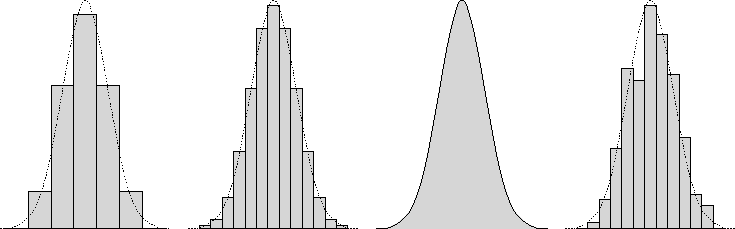
\includegraphics[width=\textwidth]{Pictures/clt}
\caption
{
%The first two graphs are the probability mass functions of $ \Binom(n,\frac{1}{2}) $ rescaled so as to show $ \pm 3 \sigma $.
%The third graph is the graph of $ y = \frac{1}{\sqrt{2\pi}}e^{-x^2/2} $.
%The fourth graph displays the relative frequencies in a random sample of $ 200 $ independent random variables with distribution $ \Binom(16,\frac{1}{2}) $.
Função de probabilidade de $\smash{\frac{S_n - n\mu}{\sigma\sqrt{n}}}$ para $S_n$ com distribuições~$\Binom(4,\frac{1}{2})$ e~$\Binom(16,\frac{1}{2})$ para valores entre $-3$ e $3$.
A área de cada retângulo é dada pela função de probabilidade.
O terceiro gráfico é a função de densidade de uma normal padrão, assim como as linhas pontilhadas.
O quarto gráfico representa as frequências relativas de $\smash{\frac{S_n - n\mu}{\sigma\sqrt{n}}}$ para $S_n$ com distribuição $\Binom(16,\frac{1}{2})$, em um experimento real com~$200$ amostras.
}
\label{fig:clt}
\end{figure}

Também podemos usar as "versões de um lado" do Teorema do Limite Central.
Dessa forma, o exemplo anterior fica simplificado:
\begin{align}
\Pb( X_1 + \dots + X_{400} \geq 215 )
& =
\Pb\Big( \frac{X_1 + \dots + X_{400}-400\cdot \mu}{\sigma \sqrt{400}} \geq 1.5 \Big)
\\ &
\approx
\int_{1.5}^{+\infty}
\tfrac{1}{\sqrt{2 \pi}}
e^{-x^2/2} \, \dd x
\\ &
\approx
0.07.
\end{align}

Se reescrevermos o Teorema do Limite Central como
\[
\Pb\Big( \mu + \frac{\sigma}{\sqrt{n}} a \leq \frac{X_1+\dots+X_n}{n} \leq \mu + \frac{\sigma}{\sqrt{n}} b \Big)
\approx
\int_a^b
\tfrac{1}{\sqrt{2 \pi}}
e^{-x^2/2} \, \dd x
,
\]
obtemos uma boa descrição do comportamento estatístico da média observada $ \frac{X_1+\dots+X_n}{n} $.
Conforme previsto pela lei das médias, a média observada está concentrada em torno de $ \mu $, mas agora podemos dizer algo mais preciso.
A média observada flutua como $ \mu + \sigma \frac{1}{\sqrt{n}} Z $, onde $ Z $ é essa "coisa" descrita por
\[
\Pb(a \leq Z \leq b) =
\int_a^b
\tfrac{1}{\sqrt{2 \pi}}
e^{-x^2/2} \, \dd x
.
\]
Variáveis aleatórias descritas em termos de integrais são chamadas de \emph{variáveis aleatórias contínuas}, que é o tema da próxima seção.
